\documentclass[12pt]{ruthesis} 
\usepackage{amsmath}
\usepackage{amssymb}
\usepackage{latexsym}
\usepackage{graphics}
\usepackage{epsfig,epsf,rotating}
\usepackage{subcaption}
%\usepackage{pictex}
\usepackage{epsf}
\usepackage{cite}
\usepackage{color}
\usepackage{theorem}
\newtheorem{proposition}{Proposition}

\theoremheaderfont{\itshape} {\theoremstyle{break}
\newtheorem{Fact}{Fact}[chapter]} \theoremstyle{break}
\newtheorem{Lem}{Lemma}[chapter] \theoremstyle{break}
\newtheorem{Thm}{Theorem}[chapter] {\theoremstyle{plain}
  \theorembodyfont{\rmfamily}  \newtheorem{Prf}{Proof}[chapter]}
{\theoremstyle{plain}
  \theorembodyfont{\rmfamily}  \newtheorem{Def}{Definition}[chapter]}

\newcommand\GRE[1]{\textcolor{green}{\textbf{#1}}}
\newcommand\RED[1]{\textcolor{red}{\textbf{#1}}}

\title{Adaptive sampling of Conformational Dynamics}
\ctitle{Adaptive sampling of Conformational Dynamics}
\author{Eugen Hruška}
%\department{Electrical and Computer Engineering}
\school{Rice University}
\degree{Doctor of Philosophy}

\committee {
        Cecilia Clementi, Thesis Director\\
Professor of Chemistry and Chemical \&
Biomolecular Engineering\and
Jose Onuchic, Chair \\
        Harry C. and Olga K. Wiess Chair of
Physics, Professor of Chemistry and
BioSciences \and
        Jason Hafner \\
        Professor of Physics \& Astronomy and
Chemistry \and
        Matteo Pasquali\\
        A. J. Hartsook Professor of Chemical and
Biomolecular Engineering, Chemistry,
Material Science and NanoEngineering 
}

\address{Houston, Texas}
\donemonth{April} \doneyear{2020} \makeindex
\begin{document}

  \begin{frontmatter}
   \pagenumbering{roman}
   %\makecover
   \maketitle
   \afterpage{\null\newpage}
\thispagestyle{empty}
\begin{abstract}

The challenge of predicting the conformation dynamics of biomolecules is at the core of our limited ability to understand many biophysical processes. This includes many questions around the causes of many diseases and biophysics theory. \emph{Adaptive sampling} is an approach to increase our ability to predict conformational dynamics. 

The challenge of effectively sampling the conformation dynamics of biomolecules is one example of a more general problem.  In terms of physics, the general problem is the accurate sampling of time-dynamics of high-dimensional stochastic systems. The high-dimensionality presents here several challenges. The high-dimensionality with a complex energy landscape prevents any simple solutions. Additionally the. 
dimensional curse. 

In the past many approaches to unravel this challenge have in the past achieved significant improvements. In the case of proteins, the timescales where we are able to predict the conformational dynamics increased by many orders of magnitudes to the millisecond scale. This illustrated the magnitude of the challenge since the current state-of-art can only small proteins and for most, larger biomolecules we are not able to predict the accurate behavior. This is not only caused by the several magnitude longer timescales but also order of magnitude larger sizes of the biomolecules.  

Considering the broad scope of the general challenge for high-dimensional stochastic system this Dissertation will focus on only improving the prediction of conformational dynamics of proteins. This restriction doesn't limit the applicability of the methods investigated to other high-dimensional stochastic systems.

First the prediction of the effectivity of different adaptive sampling strategies will be discussed. Due to significant stochasticity and protein-to-protein variation the choice of adaptive sampling strategy is not obvious. The performance for different goals varies as well. 

Second, to deepen our theoretical undertanding adaptive sampling strategies, a upper limit for the performance of any adaptive sampling strategy is developed. This theoretical upper limit allows us to understand the potential and limits of adaptive sampling.

Third, adaptive sampling is heavily dependent on software due to the thousands or millions individual steps necessary to be performed, all in an effecient fashion of a High-Performance Computer (HPC). Here we show the development of the software package \emph{ExTASY}. This framework allows to execute all the necessary steps for adaptive sampling while reducing the work-load. The innovations with ExTASY are both the high-scalability and the modularity which allow for an easy change of the adaptive sampling strategies and maintanance. 

Future developments to extend the investigated approaches to longer timescales will be addressed.

\end{abstract}



   %\include{ded}
   % star needed to make sure that the 'acknowledgments' are not included in chapter numbering
\chapter{Acknowledgments}


shatennu

vivek

request quick- summit

It has been a long way since I joined Rice as a grad student back in 2013. Over the past
(many) years I have been through a lot and, most importantly, I have met wonderful people
who, together with the unconditional support of my family, have helped me grow professionally
and personally: it just so happens that a lot of them are fellow Italians, and those
I prefer to acknowledge later in our native language.
First thing first, I would like to show my gratitude to Cecilia. She oered me the opportunity
to start such a long journey in a top-tier grad school like Rice University, which
turned out to be crucial for my professional growth. Under her advice, I got to doing high
quality research, traveling and presenting my work; also, she relentlessly encouraged me to
raise the bar by setting the example and (not to be underestimated) took me to task during
my occasional goof times. She has really been an incredible mentor.
I would also like to thank Matteo and Tolya for agreeing to sitting on my PhD defense
committee and for the insightful feedback they provided at the time of my Qualifying Exam.
Many thanks to Frank for being a great collaborator and for being always willing to help.
I would like to acknowledge all the previous and current lab mates for sharing the ride
down this very bumpy road. Mary and Wenwei were my first official lab mates, and they
helped me a lot get started with coding and other technicalities to which I had never been
really exposed before. Justin and Feliks have recently shared joys and frustration over the
last few years, especially during those less happy moments when I had no idea if I would
ever graduate.
Thanks to Dr. Gianpaolo Gobbo, Dr. Ralf Banisch and Dr. Feliks Nuske for collaboviii
rating with me on the dierent research projects.
Last but not least, I really have to thank Tim, Wei, John, Behnaam and Jesse, my
volleyball buddies. We have played so many games over the weeks, we have put in so many
hours of fun, and I have loved every minute of that. They truly are great friends to share a
volleyball court and to win Intramural Championships (twice!) with. I will miss them all.

   %\include{ack}
   \tableofcontents
   \listoffigures
   \listoftables
%   \include{ded}
  \end{frontmatter}
\pagenumbering{arabic}

\linespacing{1.7}

%\chapter{Motivation and Approach}

\section{Adaptive sampling: Motivation}
Physical systems come in many forms and shapes and show an intrinsic hierarchical organization. Molecular dynamics (MD) simulations have become indispensable for gaining
insight into molecular systems at high spatial and temporal resolutions.
However, a fundamental limitation for MD with accurate all-atom force-fields remains
the computational demand for simulating processes with long timescales. In
particular, biologically relevant processes, such as protein folding and
conformational changes, typically require simulation time orders of magnitude longer than
milliseconds. At the same time, atomic-resolution MD trajectories can currently reach
timescales on the order of milliseconds on available computational resources. 

This thesis is about solving the challenge of accurately determining the conformational dynamics of high-dimensional stochastic systems. This method is especially useful in the context of molecular dynamics (MD) of proteins. Proteins and the obtaining of accurate stationary and kinetic behavior of protein is a crucial unsolved challenge that limits our understanding of the behavior of many biological systems. Such a broad challenge requires many hierarchical approaches. Adaptive sampling is one of these approaches, which builds on top of hardware advances and software advances for the molecular dynamics engines.

\section{Outline}
 
 Overall this Dissertation resulted in several peer-reviewed publications \cite{Adstrategies2018, Extasy2016}, as well one publication under review \cite{Extasy2019}. The results obtained during this Dissertation, as well as the results in the papers, will be presented in the next chapters.
 
Chapter 2 will summarize some of the standard techniques, which will be used frequently throughout the thesis. While some of these approaches are commonly used in this field, there are also recently developed techniques that are less commonly used. The relevance of all these techniques for adaptive sampling will be highlighted. 

The theory of Adaptive sampling will be discussed in Chapter 3, as well as the derivation of the first upper limit of the adaptive sampling speed up will be shown. This novel result shows that adaptive sampling can be further improved. 
In the next chapter 4, the current strategies will be compared in a statistically robust way, and the effectiveness of each strategy will be compared for different proteins and different goals.

Chapter 5 will introduce the computational tools and software frameworks necessary to successfully and efficiently execute adaptive sampling. Due to the many subtasks, adaptive sampling contains, these practical considerations have a direct impact on the viability of adaptive sampling for solving sampling problems.

This developed software framework will be used in Chapter 6 to show the results and the accuracy which adaptive sampling can achieve for different biomolecular systems. 

A final chapter will summarize the current achievements and discuss further open questions and possible directions.




\afterpage{\null\newpage}
\chapter{Background\label{sec:background}}

\section{Proteins and Molecular Dynamics}

The behavior of a protein or any biomolecule can be relatively accurately represented by Newton's classical equations of motion of all atoms. All 3N atom coordinates, including the surrounding water solvent, are represented by $\mathbf{x}_{t}$ positions and $\mathbf{v}_{t}$ velocities. Figure~\ref{fig:proteins} shows the 3-dimensional structure of two proteins investigated in this thesis as an example. The Newton's classical equations of motion are:

$$M\ddot{\mathbf{x}_{t}}=-\nabla U(\mathbf{x}_{t})$$
The Hamiltonian $U()$ represents the all-atom force field guiding. The straightforward approach of numerically solving this equation leads to a molecular dynamics (MD) trajectory describing the motion of a protein. This Hamiltonian approximates the quantum-mechanical dynamics of the protein and is continuously improved. Increased accuracy compared to the all-atom approach would require a quantum-mechanical approach, which reduces the reachable timescales by several orders of magnitude.  In this thesis, the CHARMM22* force field \cite{Charmm22star} with modified TIP3P water was utilized.

\begin{figure}[H]
  \centering
  \begin{subfigure}[t]{0.45\textwidth}
    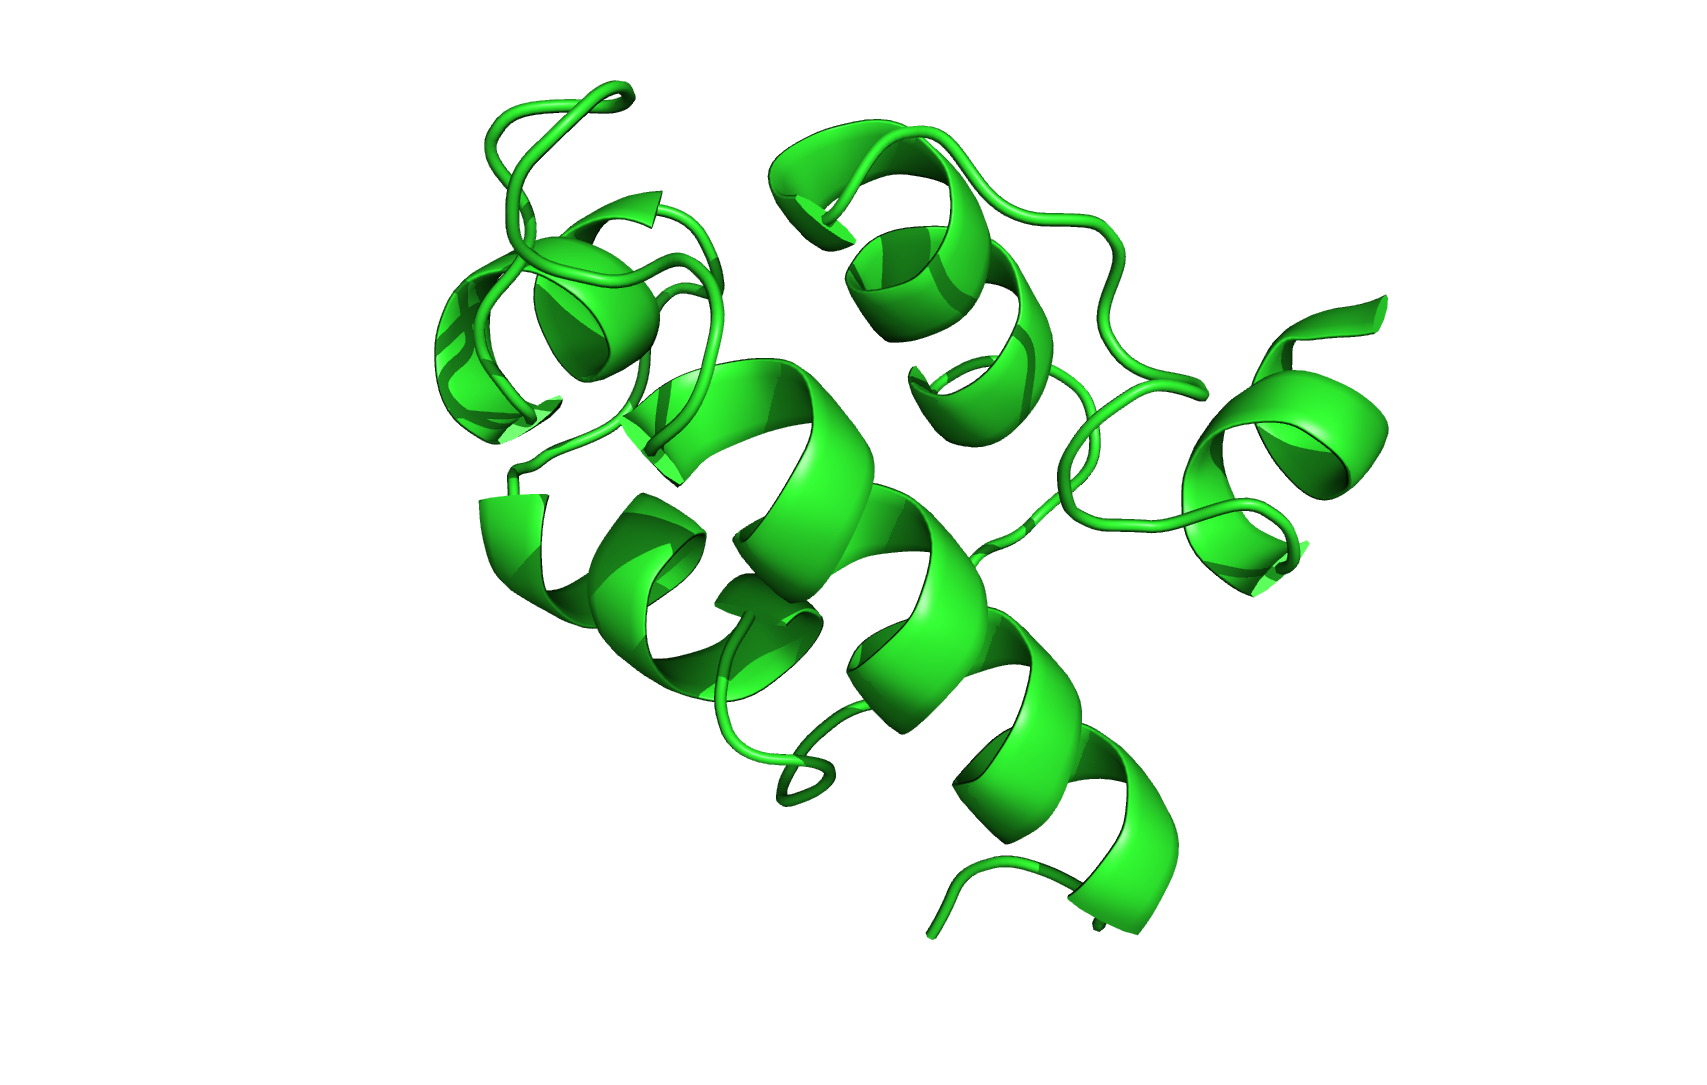
\includegraphics[width=0.9\textwidth]{figures3/lambda-repressor.png} 
  \end{subfigure}
  \begin{subfigure}[t]{0.45\textwidth}
    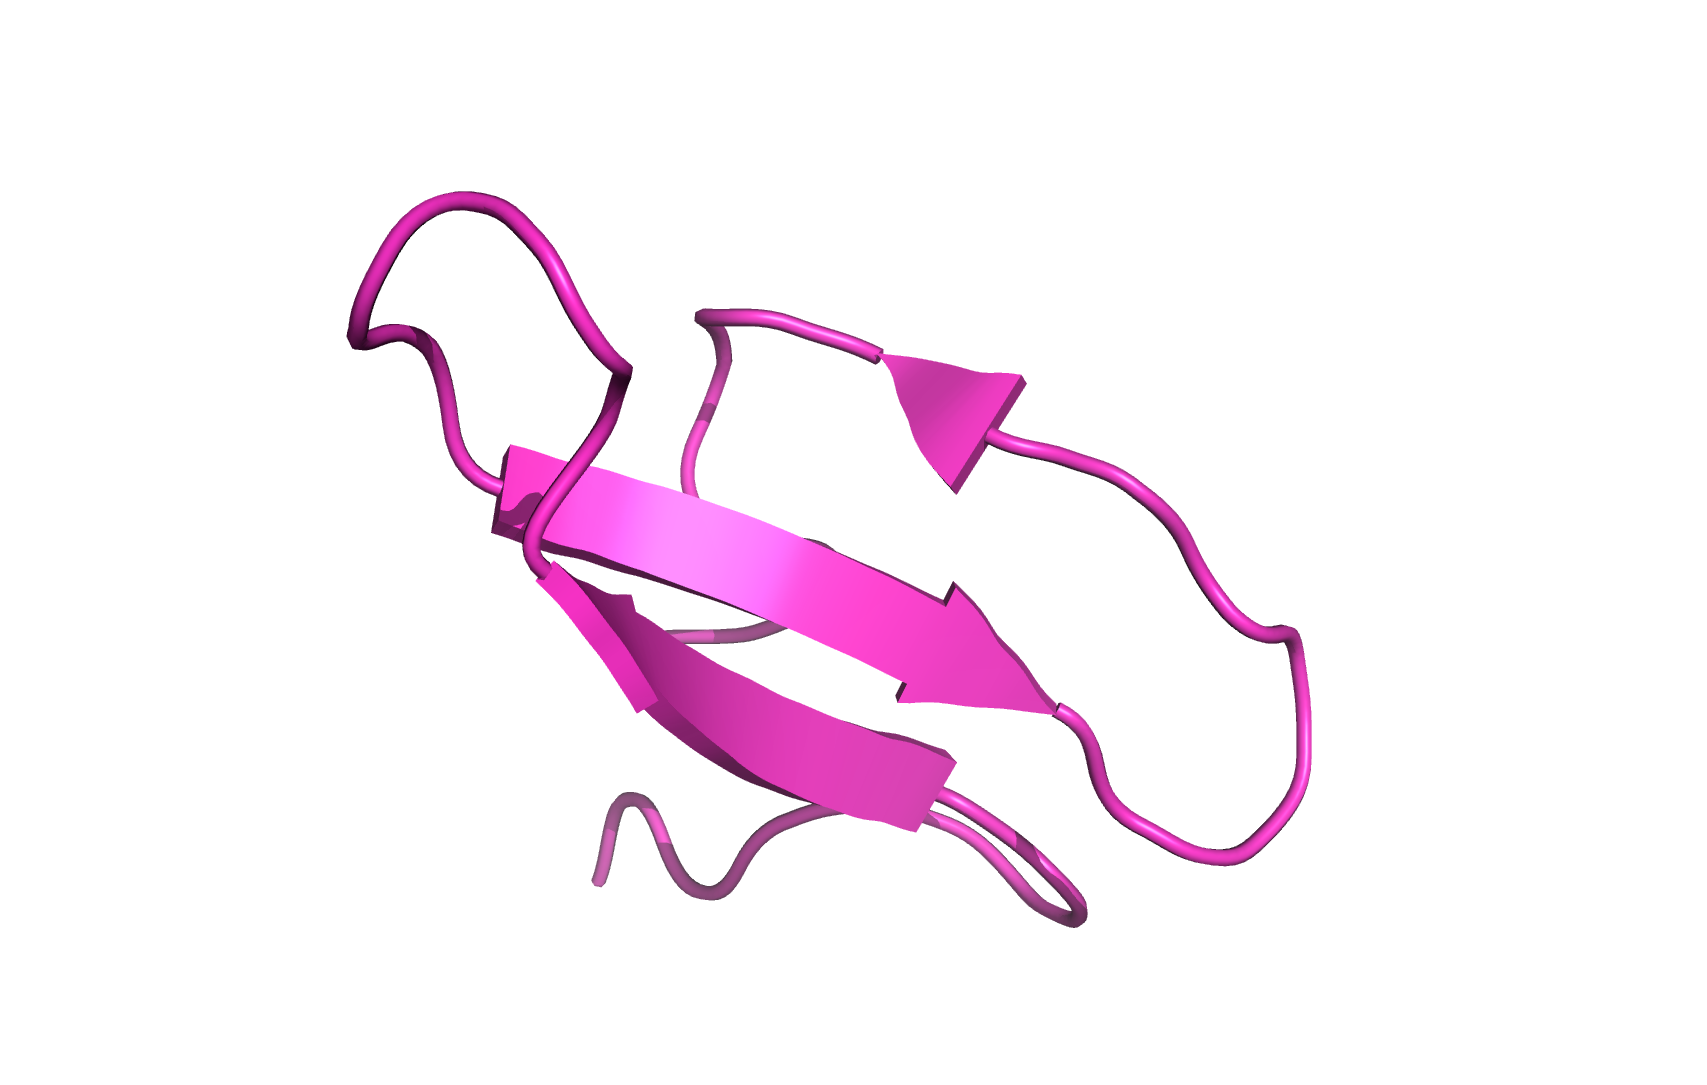
\includegraphics[width=0.9\textwidth]{figures3/ww-domain.png}  
  \end{subfigure}
  \caption{Structure of proteins $\lambda$-repressor and WW domain.}
  \label{fig:proteins}
\end{figure}


The CHARMM force field has the following Hamiltonian, which consists of terms for molecular bonds stretching, angle bending, dihedral, improper dihedral energy terms, the Urey-Bradley component, van der Waals interactions (Lennard-Jones) and Coulomb interactions. 

$$U_{\mathbf{x}}=U_{bonds}+U_{angle}+U_{dihedral}+U_{improper}+U_{UB}+U_{LJ}+U_{elec}$$

\begin{equation}
\begin{aligned}
U(\mathbf{x})={} &\sum_{bonds}K_{b}(b-b_{0})^{2}+\sum_{angles}K_{\theta}(\theta-\theta_{0})^{2}+\sum_{torsions}K_{\phi}\left(1+cos(n\phi-\delta)\right)\\
&+\sum_{impropers}k_{\omega}\left(\omega-\omega_{0}\right)^{2}+\sum_{Urey-Bradley}k_{u}\left(u-u_{0}\right)^{2}\\
&+\sum_{nonbonded}\epsilon\left[\left(\frac{R_{min,ij}}{r_{ij}}\right)^{12}-\left(\frac{R_{min,ij}}{r_{ij}}\right)^{6}\right]+\sum_{electric}\frac{q_{i}q_{j}}{\epsilon r_{ij}}
\end{aligned}
\end{equation}

Here the parameters are: $k_b$ is the bond force constant, $b-b_0$ is the atom distance from equilibrium, $k_\theta$ is the angle force constant, $\theta-\theta_0$ is the angle from the equilibrium between 3 bonded atoms, $k_\phi$ is the dihedral force constant, $n$ is the multiplicity of the dihedral function, $\phi$ is the dihedral angle, $\delta$ is the phase shift, $k_\omega$ is the improper dihedrals force constant, $\omega-\omega_0$ is the out of plane improper dihedrals angle, $R_{{min}_{ij}}$ is the constant for the Lennard-Jones potential, $r_{ij}$ is the distance between a pair of atoms and $q_{i}$ is the charge of an atom. The Urey-Bradley component serves the cross-term accounting for angle bending using 1,3 nonbonded interactions, where $k_{u}$ is the Urey-Bradley force constant, and $u-u_{0}$ is the distance between the 1,3 atoms in the harmonic potential.

One challenge of this straightforward approach of the Newton's classical equations of motion for the proteins is the relatively short timestep. The commonly used maximum timestep allowing for energy conservation and stability of the protein is between 2fs and 5f. Considering most proteins fold on timescales longer than milliseconds, this requires to simulate $10^{12}$ steps. With modern GPUs, for smaller proteins, almost 1 microsecond of molecular dynamics trajectory can be simulated per day. Special purpose hardware \cite{shaw2014anton} can simulate up to 100 microseconds of MD trajectory per simulation day, but the access to this special purpose hardware is limited. To simulate the behavior of most biomolecules for relevant processes such as protein folding and other global structural rearrangements requires timescales of around $10^{-2} - 10^{1}$s. These slow processes are associated with the rare crossing of high free energy barriers, representing a bottleneck for the MD simulations.

\section{TICA dimension reduction}

The molecular dynamics trajectory is high-dimensional, with 1000s or more individual atom trajectories. This high-dimensionality needs to be dimension-reduced to be effectively analyzed. One approach is the Time-lagged
Independent Component Analysis (TICA) \cite{TICA1-perez2013, TICA2-schwantes2013}, which includes the kinetic behavior of the protein dynamics in the dimension reduction.

The first step for TICA is the conversion of $\mathbf{x}_{t}$ trajectories into features $\mathbf{f}_{t}$ which are rotation- and translation-invariant and mean-free:
$$\mathbf{f}_{t}=F\left(\mathbf{x}_{t}-\left\langle \mathbf{x}_{t}\right\rangle \right)$$  
Some examples of features are atom distances or dihedral angles. The rotation- and translation-invariance is an usefull property since the protein dynamics is rotation- and translation-invariant.

The next step of TICA is the calculation of the correlation matrix $C_{00}$ and the time-lagged correlation matrix $C_{01}$:

$$C_{00}=\ensuremath{\mathbb{E}}_{t}\left[\mathbf{f}_{t}\mathbf{f}_{t}\right]$$
$$C_{01}=\ensuremath{\mathbb{E}}_{t}\left[\mathbf{f}_{t}\mathbf{f}_{t+\tau}\right]$$

The generalized eigenvalue problem for the correlation matrices leads to TICA, where $\mathbf{R}$ is the eigenvector matrix, and $\mathbf{\varLambda}$ is the diagonal eigenvalue matrix. 

$$C_{01}\mathbf{R}=C_{00}\mathbf{R}\mathbf{\varLambda}$$

The eigenvalues $\lambda_{i}$ allow the calculation of the timescales $t_{i}$. Generally, the dimensions with the longest timescales are relevant for biophysical applications.

$$t_{i}(\tau)=-\frac{\tau}{log\left|\lambda_{i}\right|}$$ 

The TICA dimension reduced trajectory $\varPsi(t)$ is obtained by projecting the feature trajectory on the $n$ slowest TICA eigenvectors. A kinetically meaningful state decomposition can be obtained with the commute map\cite{noe2016commute} where the slowest TICA coordinates are scaled with the corresponding timescales.
$$\varPsi_{commute}=\sqrt{\frac{t_{i}}{t_{o}}}\varPsi$$

The fraction of kinetic content allows the estimation of the dimensionality of the protein behavior \cite{noe2016commute}.
$$c_{m}=\frac{\sum_{i=1}^{m}t_{i}}{\sum_{i=1}^{n}t_{i}}$$

For non-equilibrium input $\mathbf{x}_{t}$ trajectories, the plain TICA will lead to inaccurate results due to the non-stationary distribution of the input correlation matrices. The Koopman method \cite{koopmanold,
koopman2,koopman3,koopman4, wu2017variational, Nueske2017} can be used to reduce
the non-equilibrium effects by reweighting the correlation matrices to the stationary distribution.

\section{State-free reversible VAMPnets}

One disadvantage of the TICA dimension reduction is the linearity of this approach. One non-linear dimension reduction is a deep learning approach with state-free reversible VAMPnets (SRV) \cite{Mardt2018,chen2019jcp}. The SRV method is closely related to the TICA methods, but with additional neuronal networks and backpropagation. The input to SRVs are the same protein trajectories $\mathbf{x}_{t}$ and feature trajectories $\mathbf{f}_{t}$ as for TICA. According to the schema in Figure~\ref{fig:NN} a neuronal network converts the input features $\mathbf{f}_{t}$ into a dimension reduced trajectory $\mathbf{o}_{t}$.

\begin{figure}[H]
  \centering
  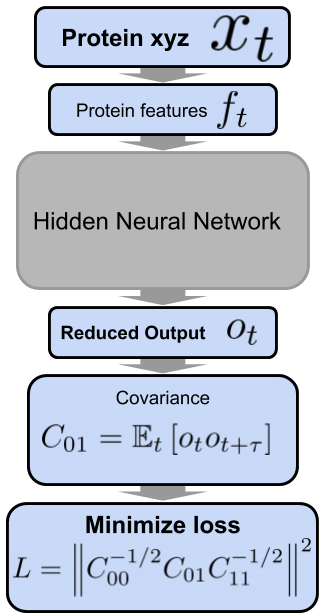
\includegraphics[width=0.4\linewidth]{figures3/NN.png}
  \caption{Schematics of the state-free reversible VAMPnets (SRV).}
  \label{fig:NN}
\end{figure}


The loss function for backpropagation to optimize the parameters of the neural network is the VAMP-2 score:
$$L=\left\Vert C_{00}^{-1/2}C_{01}C_{11}^{-1/2}\right\Vert ^{2}$$

Here the modified covariance matrix is $C_{01}=\ensuremath{\mathbb{E}}_{t}\left[o_{t}o_{t+\tau}\right]$.
The non-linear approach of SRVs allows reaching the same accuracy as TICA for shorter lag times than TICA. TICA performs better than SRVs in the case of limited data amounts.

\section{Markov state models}

The dimension reduced trajectories from TICA or SRVs are ideal for the generation of Markov state models (MSM)\cite{Noe2015}. MSM can describe the non-linear multi-state behavior of proteins. The states are commonly defined by clustering of the dimension reduced trajectory frames with k-means clustering. The clustering allows converting the dimension reduced trajectory into discrete (state) trajectories. The transitions of the discrete trajectories between states lead to the count matrix $C_{ij}$. The count matrix $C_{ij}$ indicates the number of transitions from state $i$ to state $j$ after a time lag $\tau$. The count matrix is row-normalized to obtain the transition matrix of the MSM $T_{ij}$.

The MSM behavior can be described by the eigendecomposition of the transition matrix. $\varLambda$ is the diagonal matrix of eigenvalues, and $\mathbf{U}$ is the eigenvector matrix. The slowest eigenvector represents the stationary distribution of state probabilities.

$$\mathbf{U}T=\mathbf{U}\varLambda$$


\section{Protein folding funnel}

The protein folding behavior can we visualized by the folding funnel of the energy landscape theory of protein folding\cite{bryngelson1995p}. The unfolded protein is on top of the schematic in Figure~\ref{fig:funnel}. The x-axis shows the energetic stabilization of the folded state versus the unfolded state, and the width of the folding funnel shows the conformational entropy of the states.  The folded state of the protein at the bottom of the funnel corresponds to its free energy minimum. The "rough" energy landscape represents the high-dimensional energy landscape with many local energy minimas.

\begin{figure}[H]
  \centering
  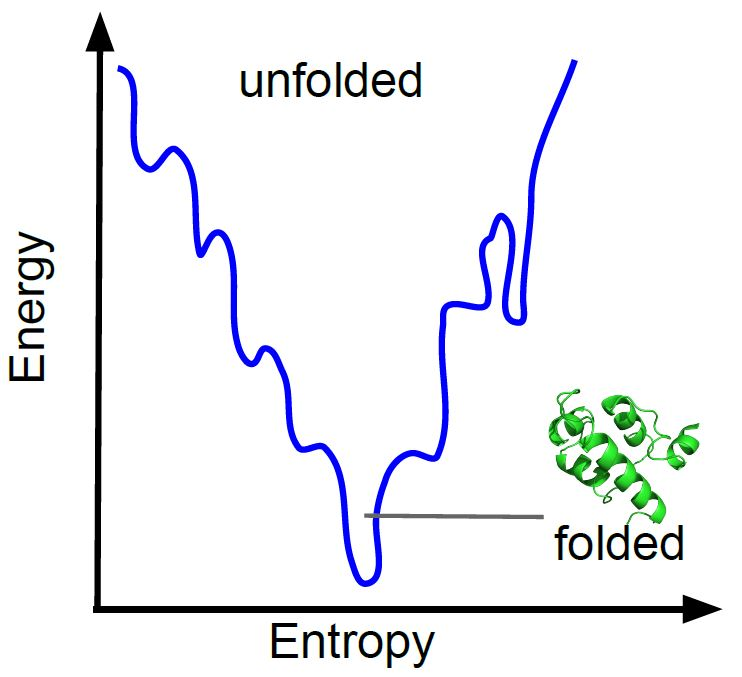
\includegraphics[width=0.4\linewidth]{figures3/folding_funnel.pdf}
  \caption{Protein folding funnel.}
  \label{fig:funnel}
\end{figure}





%\include{Introduction}
%\shipout\null

%1 -motivation, intro

% 2 - diffusion map - for dmdm for extasy 1

% 3 - theory - apper

% 4 software paper extasy1, paper extasy 2 part

% 5 applicatoon extasy paper2

% Conclusion

\include{Chapter1}    
%\shipout\null
\include{Chapter2}    
%\shipout\null
\include{Chapter3}    
%\shipout\null
\include{Chapter4}    
%\shipout\null
\include{Chapter5}    
%\shipout\null
%\include{Chapter6}    
%\shipout\null
\afterpage{\null\newpage}
\chapter{Conclusions}
\label{ch:conclude}
\emph{Adaptive sampling} increases our ability to predict conformational dynamics of high-dimensional stochastic systems or the general problem of high-dimensional stochastic systems. 
In theory adaptive sampling can increase sampling efficiency of a energy landscape by reducing the "redundant" samples. In practive the choice which sampling is "redundant" is a non-trivial and crucial step to increase the sampling efficiency of the sampling. This choice which of the sampling is "redundant" depends on the goal of the sampling and only approximations are currently possible. This reduces the effectivity of adaptive sampling to the theoretical maximum. 
In chapter \label{ch:chapter3} this theoretical maximal efficiency of adaptive sampling is derived, first time develop by the author. It is shown that this maximum efficiency depends on the goal of the sampling, wether a maximal exploration is desired or a fast folding is desired. This maximum efficiency also depends on the protein and generally increases with the complexity and size of the protein. Adaptive sampling is more efficient in a complex transition region compare to a flat transitionregion. By extrapolating we can estimate that adaptive sampling can reach a speed up of at least 10-100 for larger proteins. By comparing the theoretical maximal efficiency we can show that additional improvements in adaptive sampling strategies are possible.

In Chapter \label{ch:chapter32} we could show that different adaptive sampling strategies are superior for different goals. The \emph{cmicro} strategy is better for exploration and the \emph{cmacro} startegy is better for crossing transition barriers such as folding. This is true across different protein, but the speed up achievable with adaptive sampling depends on the complexity of the proteins. Proteins with more complex timescales are expected to have a higher speed up with adaptive sampling compared to plain molecular dynamics. The stochasticity of molecular dynamics and sampling causes the time to solution to fluctuate significant, sometimes in order of 50\%. This means a single or few folding events, commonly caused by limited computational resources, has limited statistical significance when comparing adaptive sampling with plain molecular dynamics.

The improvements of the software package \emph{ExTASY} shown in chapter \label{ch:chapter4} allow anyone to more eficiently to deploy adaptive sampling to sample any proteins. This packag ensures state-of-the-art scalability on High-Performance Computers and the modularity ensures the maintainalibity and user-friendly extensibility.

The application of \emph{ExTASY} in Chapter \label{ch:chapter5} shows that adaptive sampling reaches the promised speed ups for proteins up to size of 72 residues. For these proteins not only the folded state is recovered, but also conformational dynamics. Extending to larger proteins is only limited by computational resourced.

Together the results in this Disseration all contribute to better understanding of adaptive sampling. With better and better understood  adaptive sampling we are able to estimate the conformational dynamics of biomolecules for even longer timescales.  While the improvements shown are significant, additional improvements are necessary to reach even longer timescales. Adaptive sampling shows promise to contribute futher in reaching longer timescales, due to the significant gap between the practically reached speed up and the theoretically maximal speed up. Also the impacts of new question such as the asynchronous execution are unanswered.

While all the applications here are on biomolecules, the adaptive sampling works as well on the general problem of high-dimensional stochastic systems. For example, inorganic materials or deep learning where the loss function can represent the high-dimensional energy landscape.

Additional research of adaptive sampling could allow us to develop more effective adaptive sampling strategies or adaptive sampling strategies optimized for new goals, such as accurate mean first passage times. This dissertation is a starting point for further investigations.

   

\appendix

%\include{append-a}
%\appendix
%\addcontentsline{toc} {chapter}{\numberline {}Appendix}
%\include{append-a}
%\include{append-b}
%\addcontentsline{toc} {chapter}{\numberline {}Bibliography}{}
%\include{PhD_bib}

\bibliographystyle{naturemag}
\bibliography{thesis_main}
\end{document}
